\documentclass[compress, hyperref={pdfpagelayout=SinglePage}]{beamer}

%Para digitar e compreender em portugues os comandos
\usepackage[brazil]{babel}
\usepackage[utf8]{inputenc}

\usepackage{verbatim}

%Remove Warnings de tamanho de letra.
\usepackage{lmodern} 

%Pacote de cores
\usepackage{color}
\usepackage{xcolor}   
\usepackage{colortbl}

\definecolor{verde}{rgb}{0.88,1,1}
\definecolor{azul}{rgb}{0.62, 0.85, 1}
\definecolor{amarelo}{rgb}{1, 0.95, 0.62}
\definecolor{vermelho}{rgb}{0.85, 0, 0.075}
\definecolor{roxo}{rgb}{0.69, 0.57, 0.86}


%Seleciona um tema para usar na apresentação.
\usetheme{CambridgeUS}

%Remove a barra de navegacao(bugada) do Beamer.
\setbeamertemplate{navigation symbols}{}

%Permite utilizar hyperlinks externos
\usepackage{hyperref}
\hypersetup{linkcolor=blue,citecolor=blue,filecolor=black,urlcolor=MidnightBlue} 

%Primeiro paragrafo eh identado
\usepackage{indentfirst}

%Otimizacao de tabelas/espacamento/pdf
\usepackage{array}  
\usepackage{microtype}
\usepackage{cmap}
\usepackage[T1]{fontenc}

%Parece letra times
\usepackage{times}
\usepackage{graphicx}


\title[Data Science]{Machine Learning 101}
\author{Autor: Dirso}

\begin{document}

	\begin{frame}
		\titlepage
	\end{frame}
	
	\section*{Sumário}

\begin{frame}{Sumário}
  \tableofcontents
\end{frame}

	
	\section*{Apresentação}

\begin{frame}	
	\begin{block}{Pessoal}	
		\begin{itemize}
			\item Adilson Khouri,  jogador de Magic the Gathering, nerd, apaixonado por computação, machine learning, brasileiro mas não sei jogar futebol nem sambar!
		\end{itemize}
		\begin{figure}[!htb]
			\centering	  				
			
\includegraphics[height=5cm, width = 7cm]{./pic/AdilsonArgentina.jpg}
			\caption{Eu na Argentina!}
			\label{fig_adilson_argentina}
		\end{figure}
		
	\end{block}
\end{frame}
			
\begin{frame}	
	\begin{block}{Formação Acadêmica}
		 \begin{itemize}
			  \item Bacharel em Sistemas de Informação (2011 - USP)
			  \item Mestre em Sistemas de Informação (2016 - USP)
			  \item Doutorando em Sistemas de Informação (cursando - USP)
		  \end{itemize}
	\end{block}
\end{frame}

\begin{frame}	
	\begin{block}{Experiência de Mercado}
		\begin{itemize}
			\item Programador na consultoria Arbit (2010-2011)
			\item Programador Itaú-Unibanco (2011-2013)
			\item Cientista de dados Sr. PagSeguro (2016 - 2018)
			\item Cientista de dados Sr. NuvemShop (Atual)
			\item Professor de Programação - SENAC (Atual)
		\end{itemize}
	\end{block}
\end{frame}

	
	\section{Processo de Data Science}

\begin{frame}	
	\begin{block}{Processo de Data Science}	
		\begin{figure}[!htb]
			\centering	  				
			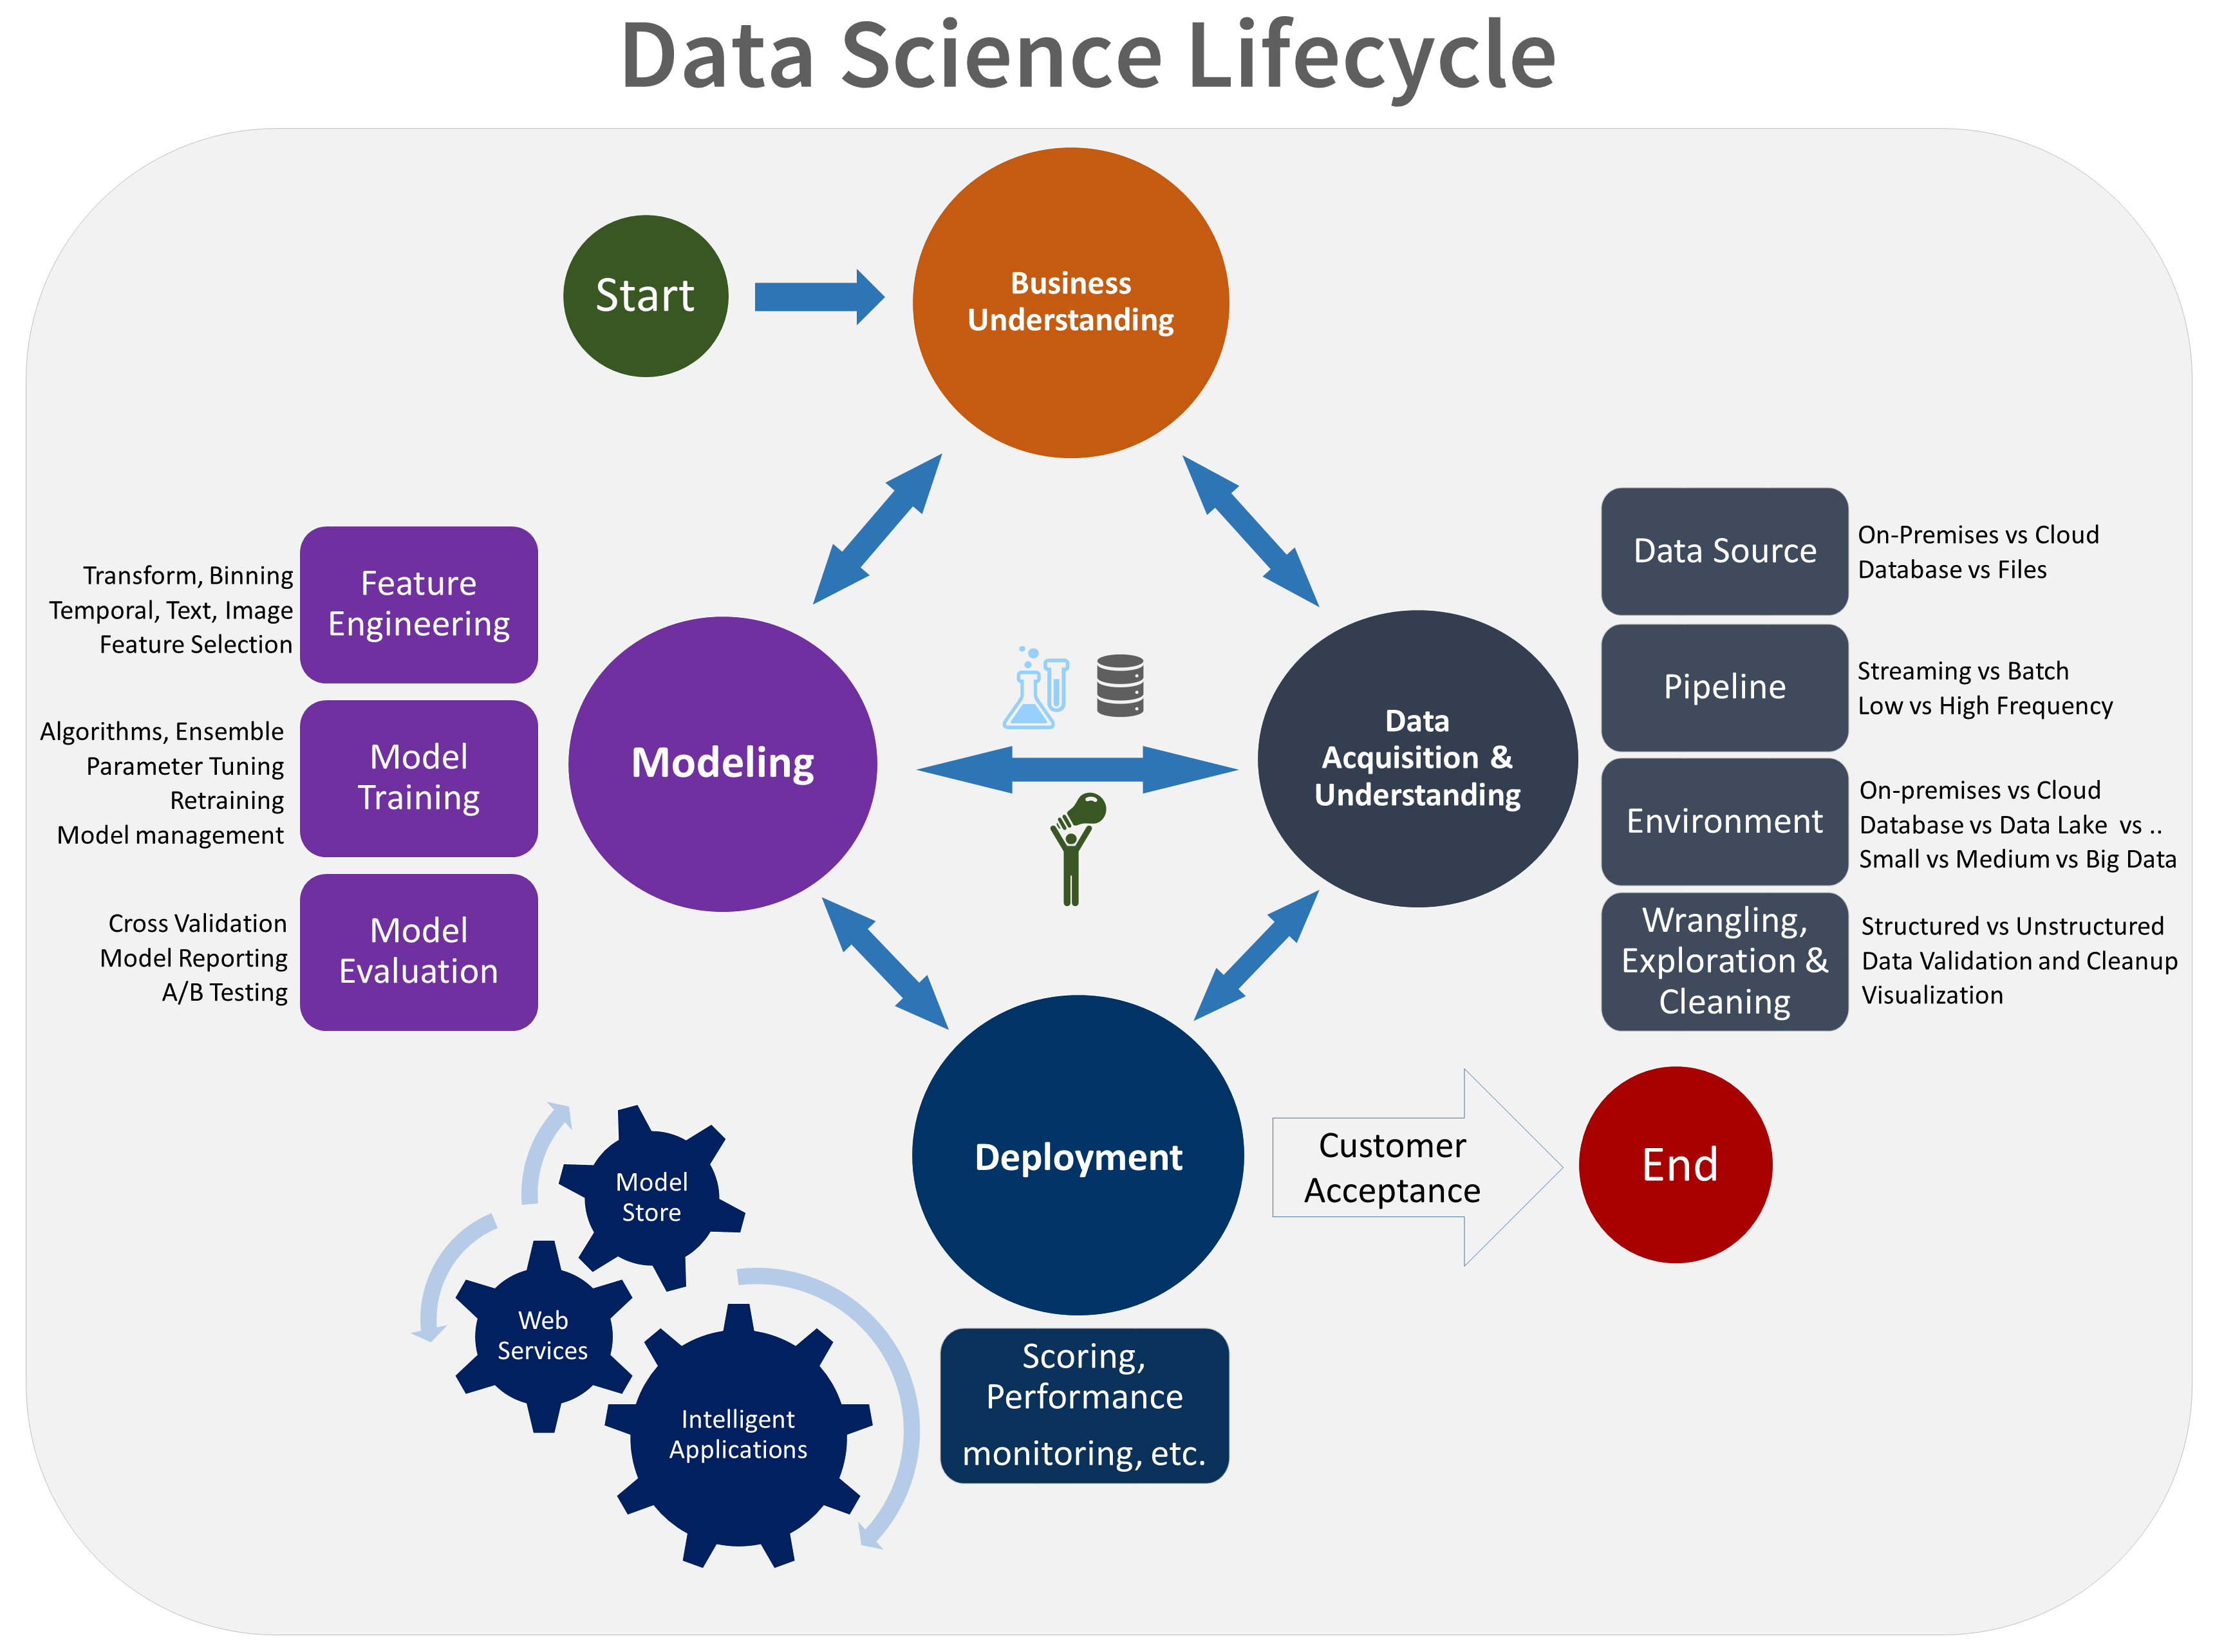
\includegraphics[height=6cm, width = 10cm]{./pic/dsprocess.png}
			\caption{Obtido em: https://docs.microsoft.com/en-us/azure/machine-learning/team-data-science-process/overview}
			\label{fig_ds_process}
		\end{figure}	
	\end{block}
\end{frame}

	
	\section{Processo Modelagem}

\begin{frame}	
	\begin{block}{Processo Modelagem}	
			\begin{itemize}
				\item Existem muitos processos para usar na área de big data, um dos mais simples e práticos é o  \href{http://www.bigdatabusiness.com.br/se-voce-se-interessa-por-big-data-precisa-entender-o-crisp-dm/}{\color{blue}{CRISP-DM}} 
			\end{itemize}
			\begin{figure}[!htb]
				\centering	  				
					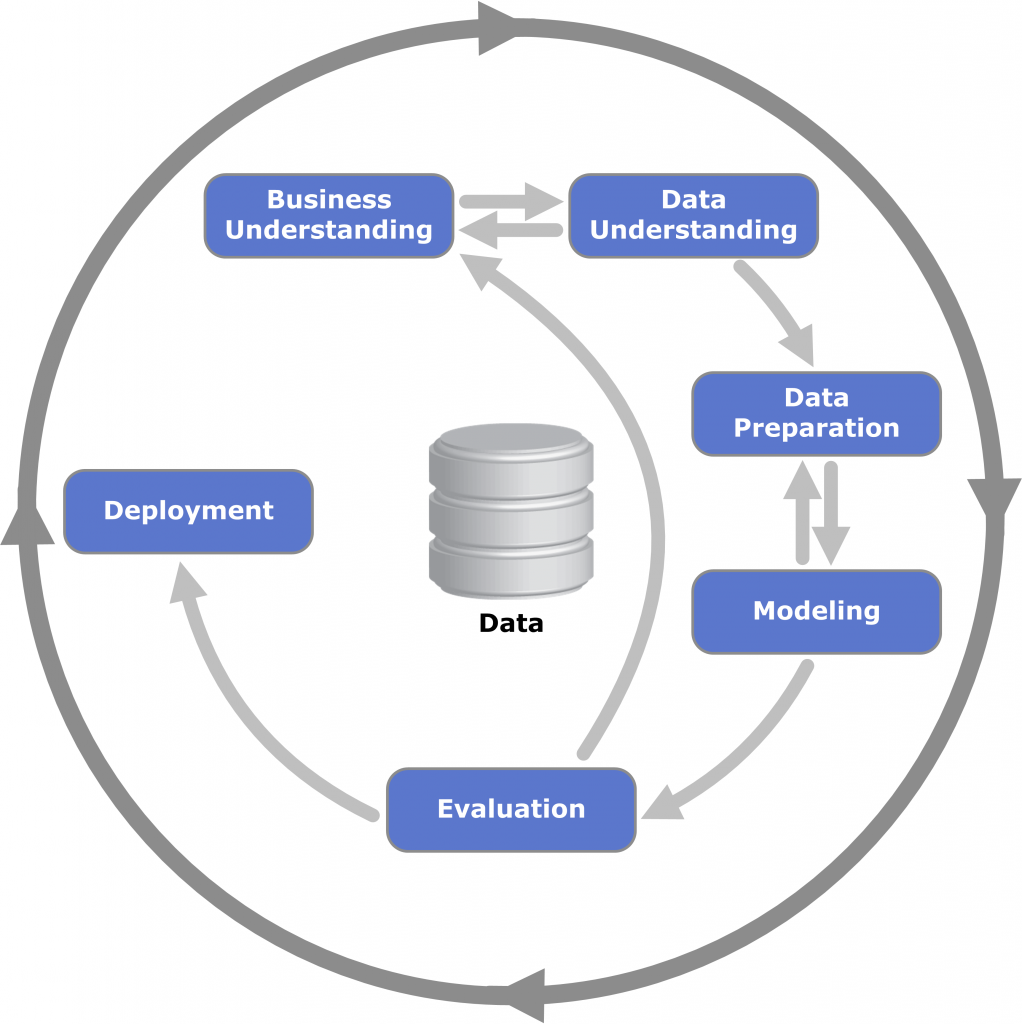
\includegraphics[height=6cm, width = 10cm]{./pic/CRISPDM.png}
				\caption{Processo CRISP-DM}
				\label{fig_brincadeira}
		\end{figure}	
	\end{block}
\end{frame}

\begin{frame}	
	\begin{block}{Processo Modelagem}	
			\begin{itemize}
				\item Entendimento de negócio
				\item Entendimento dos dados
				\item Preparação dos dados 
				\item Modelagem
				\item Avaliação do modelo
				\item Deploy
			\end{itemize}
	\end{block}
\end{frame}

\begin{frame}	
	\begin{block}{Método científico}	
			\begin{figure}[!htb]
				\centering	  				
					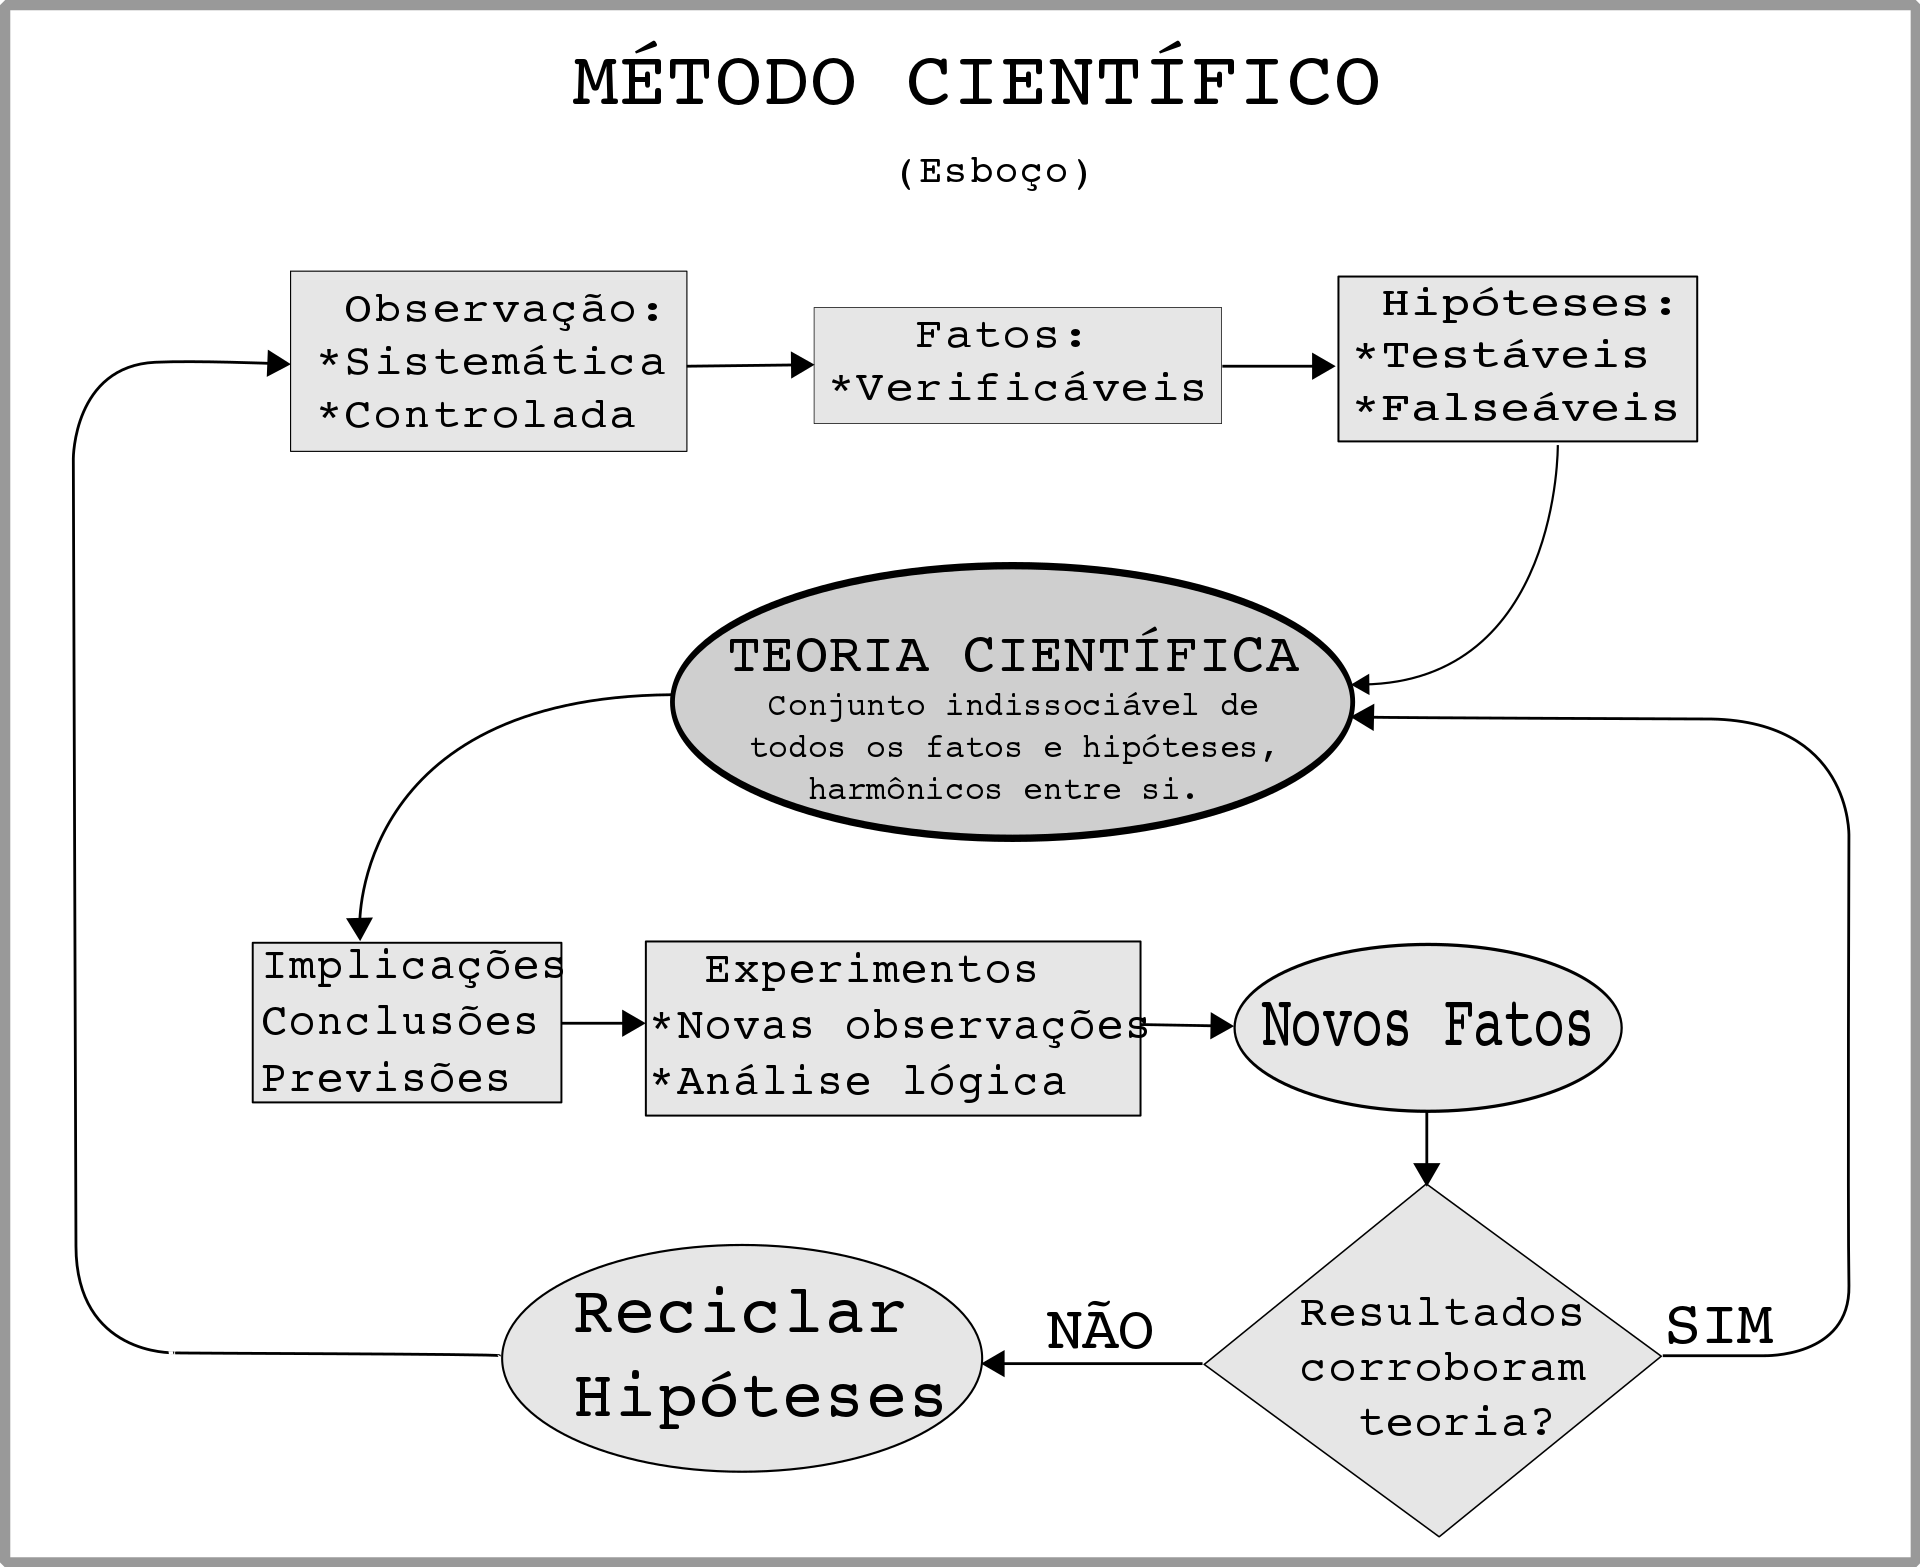
\includegraphics[height=6cm, width = 10cm]{./pic/metodoCientifico.png}
				\caption{Método científico}
				\label{fig_brincadeira}
		\end{figure}	
	\end{block}
\end{frame}

\begin{frame}	
	\begin{block}{Método científico}	
			\begin{itemize}
				\item Então método científico nos impede de cometer erros?
			\end{itemize}
	\end{block}
\end{frame}

\begin{frame}	
	\begin{block}{Método científico}	
			\begin{itemize}
				\item Por que Dirso ficou doente na Argentina em 2018?
			\end{itemize}
			\begin{figure}[!htb]
				\centering	  				
					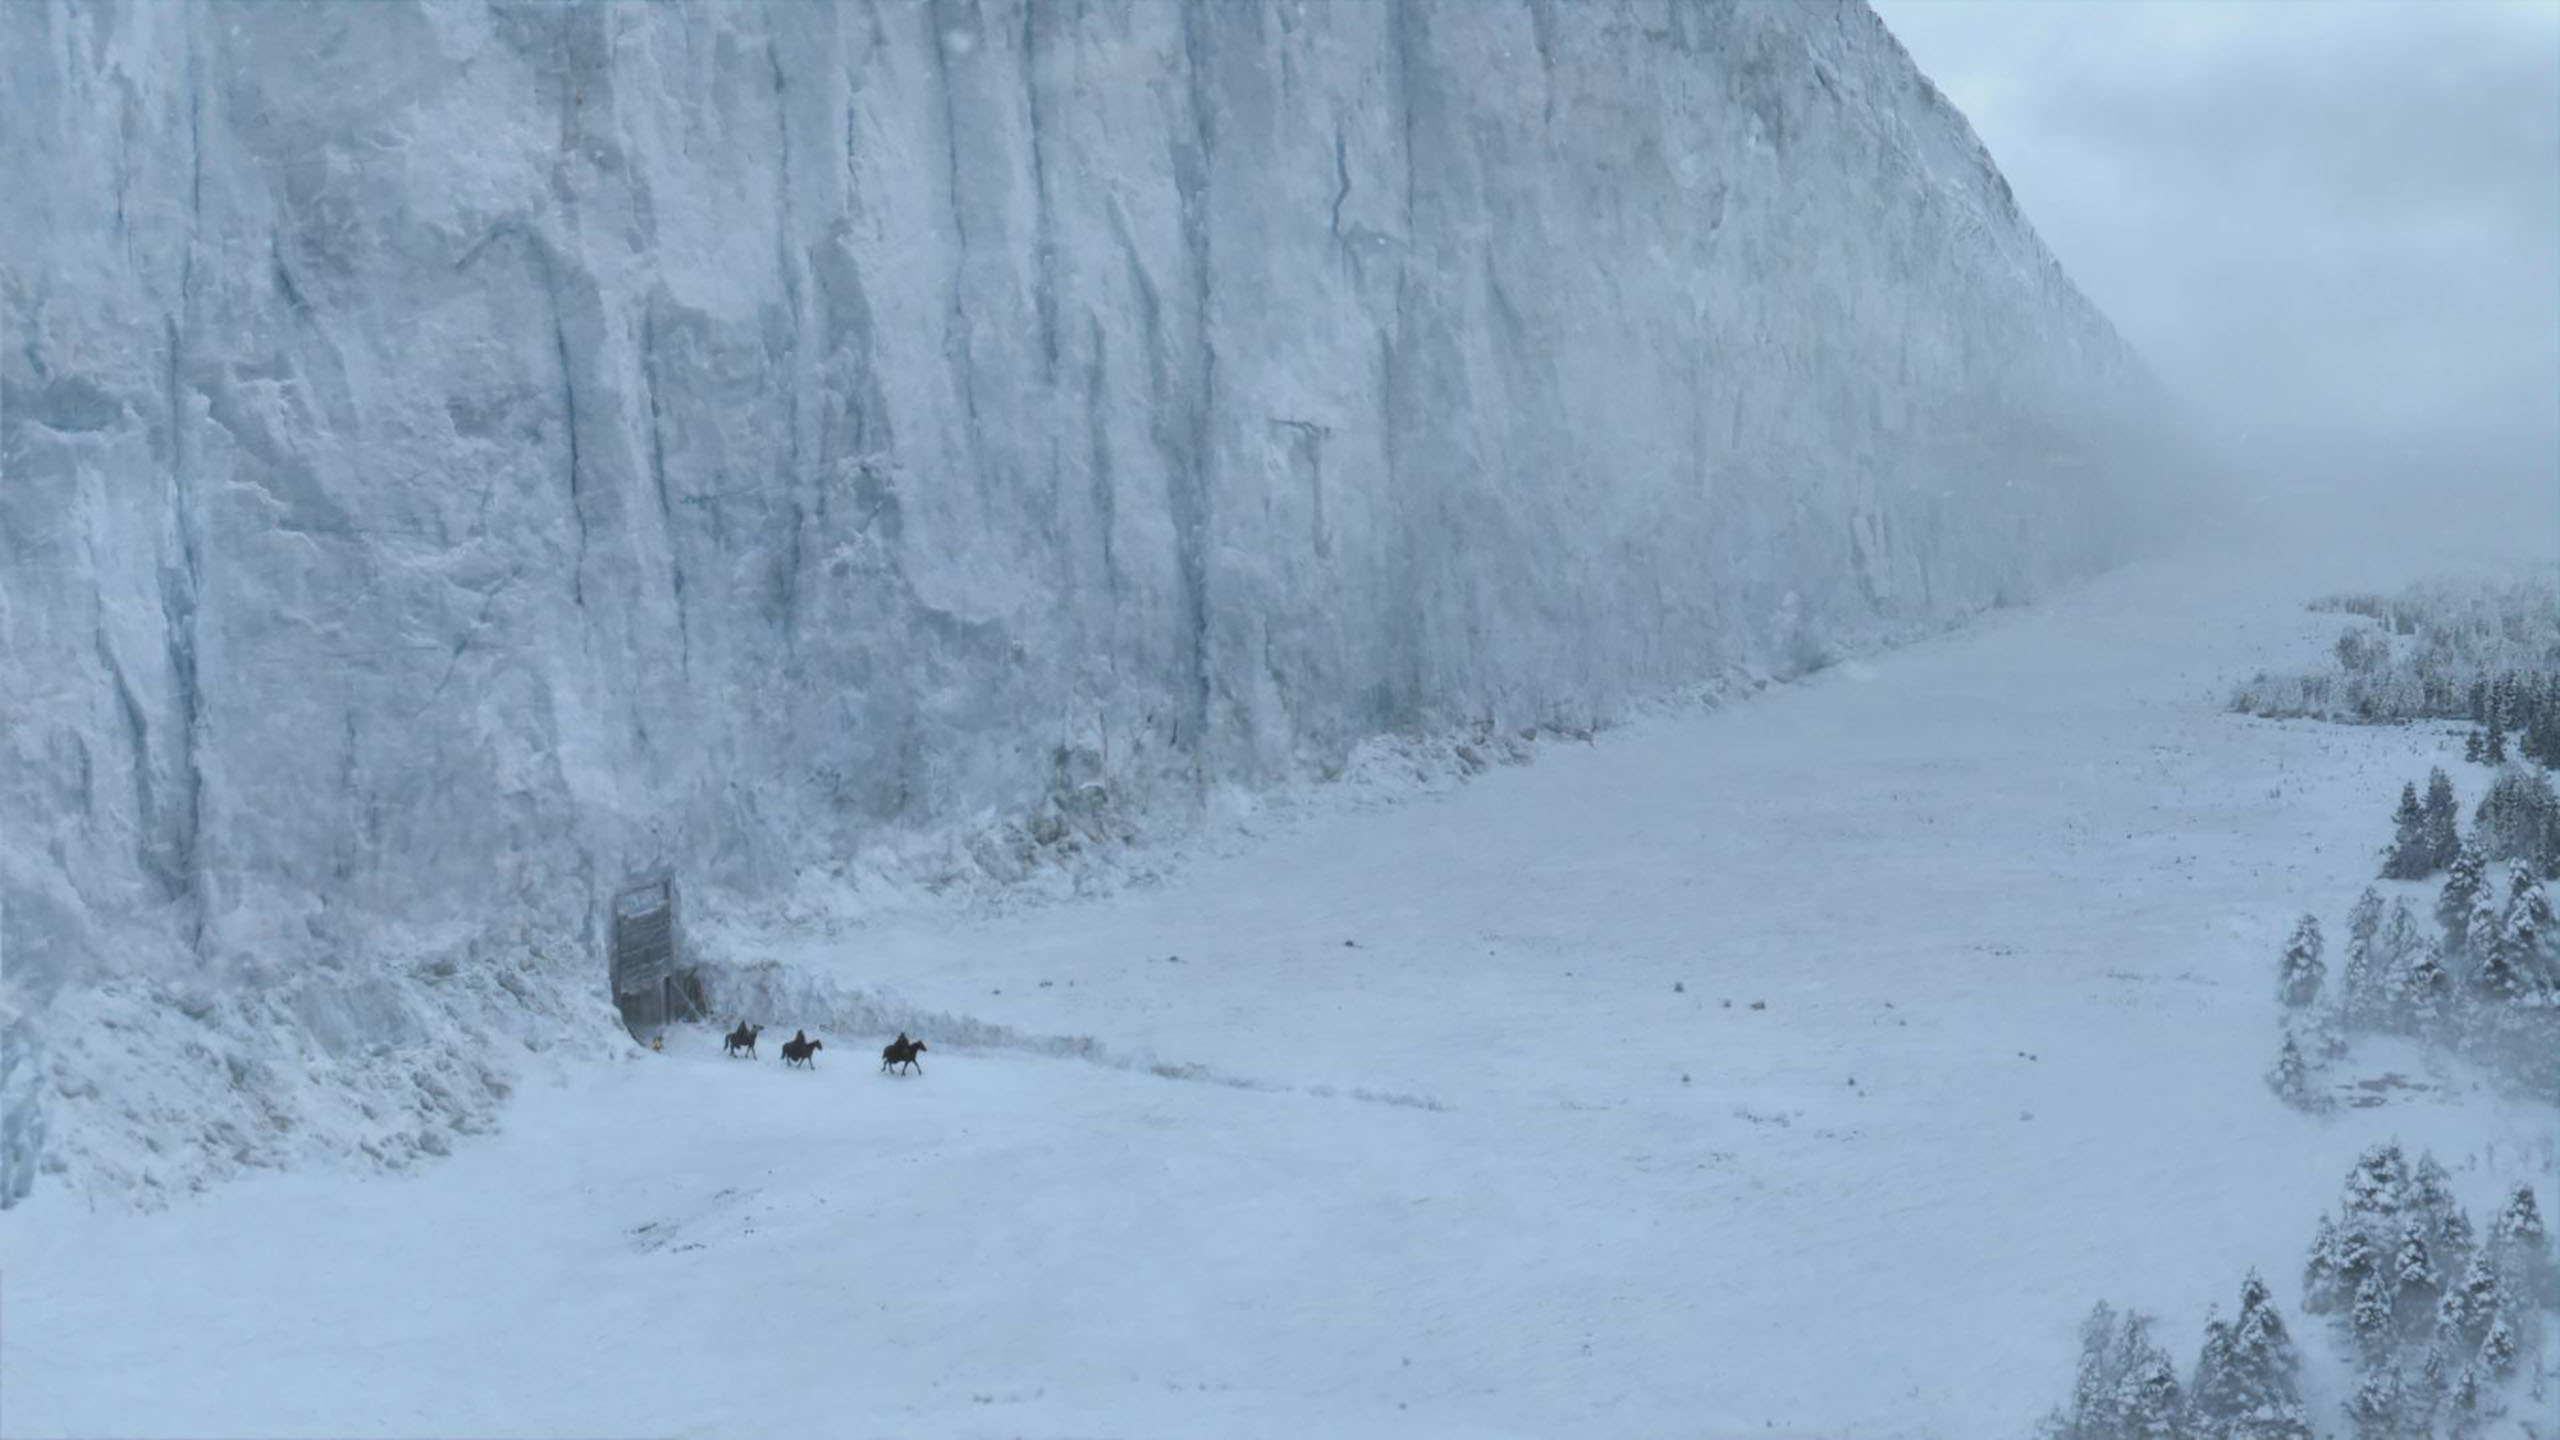
\includegraphics[height=6cm, width = 10cm]{./pic/wall.jpg}
				\caption{Na minha cabeça a Argentina é tipo wall de game of thrones!!!!}
				\label{fig_brincadeira}
		\end{figure}	
	\end{block}
\end{frame}

\begin{frame}	
	\begin{block}{Método científico}	
			\begin{itemize}
				\item Como essas duas perguntas se relacionam com essa apresentação?
			\end{itemize}
	\end{block}
\end{frame}


			
	
	\section{PagSeguro}

\begin{frame}	
	\begin{block}{PagSeguro: Risco e modelagem}	
		\begin{itemize}
			\item Atuação em modelo para previsão de chargeback em transações financeiras
			\item Criação de regras de risco para incrementar o modelo
			\item Clusterização de vendedores para agrupar por tipo de risco de chargeback
			\item Criação de árvore CART para determinar regras novas para aumentar o grau de discriminação do modelo
			\item Criação de modelo para detecção de anomalias em clientes - baseado em intervalo de confiança e aproximação por Gaussiana 
		\end{itemize}		
	\end{block}
\end{frame}


\begin{frame}	
	\begin{block}{PagSeguro: Consultor interno de data science}	
		\begin{itemize}
			\item Relatório de market share para área de produtos da empresa determinar onde investir mais dinheiro em propaganda
			\item Relatório para avaliação de carrinhos abandonados da empresa
		\end{itemize}
	\end{block}
\end{frame}
	
	\section{NuvemShop}

\begin{frame}	
	\begin{block}{Pagamentos}	
		\begin{itemize}
			\item Avaliação de variáveis para discriminar clientes (quais vão, ou não, ativar a assinatura)
			\item Levantamento de variáveis, treinamento e validação de modelo para prever pagamento de assinatura
			\item Palestra sobre erros comuns em amostragem
			\item Automatização de extrator de dados (12h semanais para 20min semanais)
		\end{itemize}		
	\end{block}
\end{frame}


	
	\section{Amostragem - principais erros}

\begin{frame}	
	\begin{block}{Amostras viesadas}	
		\begin{itemize}
			\item Precisamos de informação precisa e sem viés para tomarmos boas decisões.
			\item Se você ``cria conhecimento' ou ``toma decisões'' usando informação viesada você não está sendo \# datadriven
			\item A probabilidade de tomar decisões ruins aumenta... e decisões ruins costumam ser caras...
		\end{itemize}		
	\end{block}
\end{frame}

\begin{frame}	
	\begin{block}{processo de KDD}	
		\begin{figure}[!htb]
			\centering	  				
			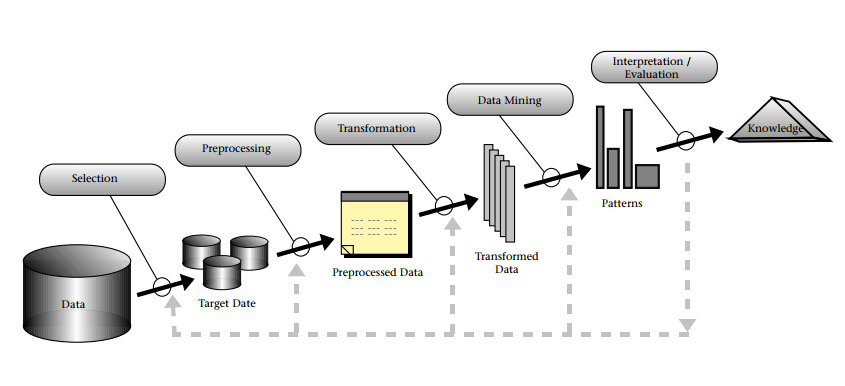
\includegraphics[height=5cm, width = 12cm]{./pic/kddprocess.jpg}
			\caption{Processo de KDD}
			\label{fig_kdd_process}
		\end{figure}
		\begin{itemize}
			\item Se você cometer um erro durante a etapa de: ``seleção'' os passos seguintes e suas conclusões estarão erradas.
		\end{itemize}
	\end{block}
\end{frame}

\begin{frame}	
	\begin{block}{Amostragem 101}	
		\begin{figure}[!htb]
			\centering	  				
			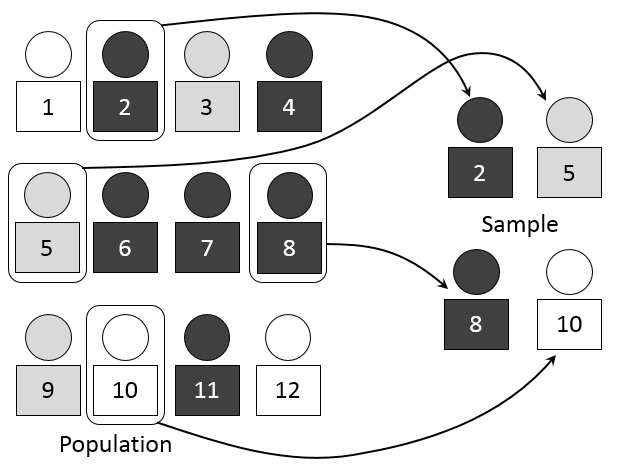
\includegraphics[height=5cm, width = 12cm]{./pic/sampling.png}
			\caption{Overview de amostragem}
			\label{fig_sampling}
		\end{figure}
		\begin{itemize} 
			\item O subconjunto (amostra) de elementos deve ser representativa da população.
		\end{itemize}
	\end{block}
\end{frame}

\begin{frame}	
	\begin{block}{Bias de auto seleção}	
		\begin{itemize} 
			\item Suponha um estudo estatístico sobre detalhes íntimos da sexualidade de estudantes em universidades. Algumas pesssoas provavelmente vão mentir.
			\item Uma pesquisa online sobre quem gosta de usar computador.
			\item Em ambos as pessoas selecionadas vão terão seus comportamentos diferentes da população geral.
		\end{itemize}
	\end{block}
\end{frame}


\begin{frame}	
	\begin{block}{Undercoverage Bias}	
		\begin{itemize} 
			\item Digest em 1936 fez uma pesquisa eleitoral que previa vitória larga do candidato Lando em relação ao candidato Roosevelt. Roosevelt ganhou com uma margem larga, a pesquisa era feita por telefone, na época pessoas pobres (maioria da população que era a favor de Roosevelt) não tinha telefone. Essa foi uma das causas do erro estatístico.
		\end{itemize}
	\end{block}
\end{frame}

\begin{frame}	
	\begin{block}{Survivorship Bias}	
		\begin{itemize} 
			\item Ocorre quando as observações estudadas no fim da investigação são não aleatórias em comparação as presentes no começo da observação.		
		\end{itemize}
	\end{block}
\end{frame}


\begin{frame}	
	\begin{block}{Survivorship Bias}	
		\begin{itemize} 
			\item Exemplo da segunda guerra mundial (tiros em avião)
		\end{itemize}
	\end{block}
\end{frame}


	
	\section{Engenharia de features}

\begin{frame}	
	\begin{block}{Engenharia de features}
		\begin{itemize}
			\item Modelos usam muitas variáveis para tomar decisões
			\item Encontrar boas variáveis é parte fundamental para um modelo
			\item Citar exemplo de variáveis de transações financeiras
			\item Citar exemplo de variáveis de pagamento de assinaturas
			\item Citar exemplo de um classificador de brasileiros e peruanos			
		\end{itemize}		
	\end{block}
\end{frame}


	
	\section{Overview de modelos}

\begin{frame}	
	\begin{block}{Modelos}	
			\begin{figure}[!htb]
			\centering	  				
			
\includegraphics[height=6cm, width = 10cm]{./pic/AI.png}
			\caption{Brincadeira, cada modelo trabalha internamente de uma forma distinta!}
			\label{fig_brincadeira}
		\end{figure}	
	\end{block}
\end{frame}

\begin{frame}	
	\begin{block}{Modelos}	
		\begin{itemize}
			\item Modelos tomam decisões baseados em diversas variáveis para, entre outras coisas, classificar dados
			\item Quem são peruanos e quem são brasileiros nessa sala?
			\item Há modelos para classificar em duas classes ou mais.
		\end{itemize}			
		\begin{figure}[!htb]
			\centering	  				
			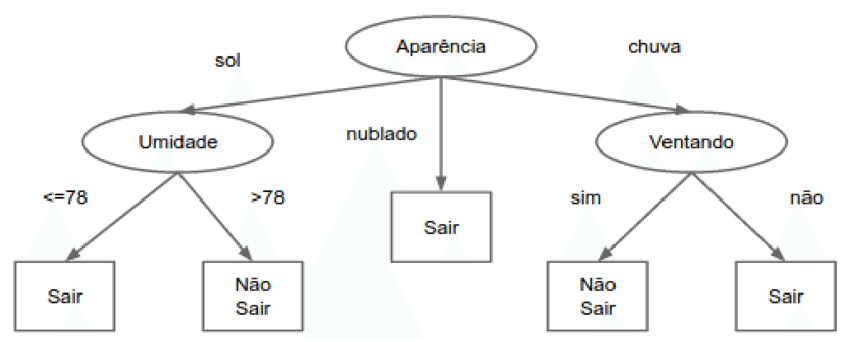
\includegraphics[height=4cm, width = 10cm]{./pic/arvore.png}
			\caption{Exemplo de árvore de decisão para sair de casa}
			\label{fig_Arvore}
		\end{figure}	
	\end{block}
\end{frame}
	
	\section{Treinamento de modelos}

\begin{frame}	
	\begin{block}{Treinamento}	
		\begin{itemize}
			\item O processo de treinamento é único para cada modelo mas a forma como se treina um modelo é parecida
			\item Os dados são dividos em treino (70\%) e teste (30\%)
			\item O conjunto de treino é apresentado ao modelo com os rótulos de cada observação
			\item Tipicamente usa-se uma validação cruzada para treinar o modelo
		\end{itemize}		
	\end{block}
\end{frame}

\begin{frame}	
	\begin{block}{Validação}	
		\begin{itemize}
			\item O modelo é validado com o conjunto de teste, o qual não deve exibir os rótulos para o modelo
		\end{itemize}
				\begin{figure}[!htb]
			\centering	  				
			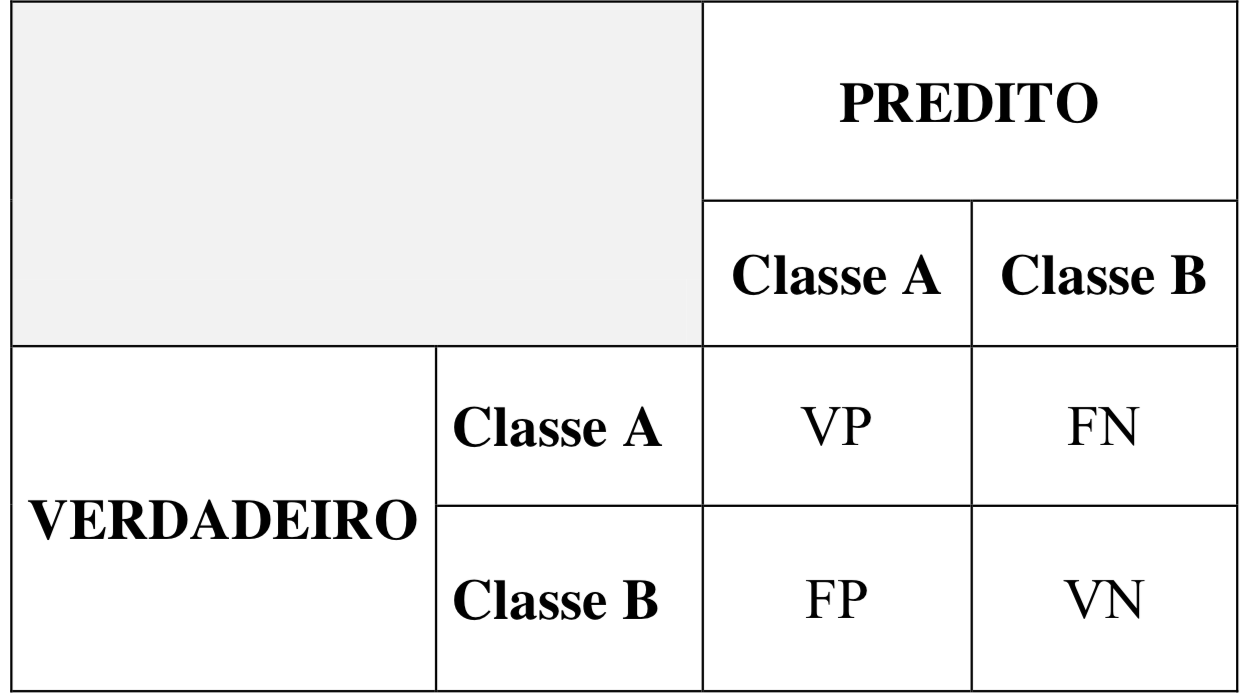
\includegraphics[height=4cm, width = 10cm]{./pic/matrizConfusao.png}
			\caption{Obtido no link: \href{http://www.scielo.br/pdf/eagri/v33n6/19.pdf}{Scielo} }
			\label{fig_matriz_confusao}
		\end{figure}	
	\end{block}
\end{frame}

\begin{frame}	
	\begin{block}{Validação - outras métricas}	
		\begin{itemize}
			\item Se usarmos a matriz de confusão acima podemos obter outras métricas
			\item Citar o problema das classes de seller (relacionar com $F1$)
		\end{itemize}
		\begin{equation*}
			\setlength{\jot}{10pt}
				\begin{aligned}
					\textrm{Precision} &= \frac{TP}{TP + FP} \\
					\textrm{Recall} &= \frac{TP}{TP + FN} \\
					\textrm{F1} &= 2 * \left(  \frac{\textrm{Precision}  * \textrm{Recall}}{\textrm{Precision}  + \textrm{Recall}} \right)
				\end{aligned}
		\end{equation*}
	\end{block}
\end{frame}
	
	\section{Ferramentas}

\begin{frame}	
	\begin{block}{Ferramentas}	
		\begin{itemize}
			\item Na teoria pode-se usar qualquer linguagem de programação para trabalhar com Data Science
			\item Na prática usa-se, majoritariamente, a plataforma R e a linguagem Python (com alguns pacotes científicos)
			\item \href{http://scikit-learn.org/stable/}{\color{blue}{Sci-kit learn}}
			\item \href{https://www.r-bloggers.com}{\color{blue}{blog sobre R}}
						
		\end{itemize}		
	\end{block}
\end{frame}

\begin{frame}	
	\begin{block}{Hands on}	
		\begin{itemize}
			\item Treinar modelo em Python com o time.
		\end{itemize}		
	\end{block}
\end{frame}

	
	\section*{Agradecimentos}

\begin{frame}
	\begin{block}{Fim!}
		Agradeço a Laura por me dar a possibilidade de fazer a apresentação e agradeço a vocês por assistirem :)
	\end{block}
\end{frame}


	\section{Contato}

\begin{frame}	
	\begin{block}{Contato}	
		\begin{itemize}
			\item E-mail:  $adilson.khouri.usp@gmail.com$
			\item Phone: $+55 11 9444-26191$
			\item \href{https://www.linkedin.com/in/adilson-khouri-51893918/}{\color{blue}{Linkedin}}
			\item \href{http://lattes.cnpq.br/2654721135214993}{\color{blue}{Curriculum Lattes}}
			\item \href{https://github.com/khouri/Apresentacao_Cusco}{\color{blue}{Código fonte GitHub}}
		\end{itemize}
	\end{block}
\end{frame}


\end{document}